\section{Características de la solución}
\label{sec:caracteristicas-solucion}
La solución consiste en incorporar un módulo en NEURONE \parencite{gonzalez2017neurone} que clasifique y prediga de forma continua del desempeño de búsqueda de los estudiantes de enseñanza básica en un curso de alfabetización informacional, específicamente en el tema de investigaciones en línea\footnote{\traduccionlibre} (\ingles{online inquiry}). 

Los datos son recopilados y almacenados por NEURONE, estos datos provienen de registros del proceso de buscar información en línea en un sistema cerrado, los cuales son: historial de navegación, consultas realizadas, movimientos del \ingles{mouse}, escritura por teclado, número de \ingles{clicks} y tiempos de permanencia en páginas \ingles{web}. Además, se conoce con anticipación los documentos y párrafos ideales a seleccionar por parte de los estudiantes.

La información de los estudiantes y el resultado de las evaluaciones definen una buena o mala navegación. La plataforma en particular debe predecir de forma continua el desempeño de los estudiantes a partir de su comportamiento de búsqueda de información actual.

El módulo propuesto hará uso de Spark, el cual se conectará con el sistema NEURONE, funcionando como una extensión del mismo, consultando su base de datos, alimentando y perfeccionando el modelo. El ciclo de construcción, evaluación y optimización del modelo se describe en la Figura 3.1, donde el modelo está en una continua optimización.


\begin{figure}[htb]
	\centering
	%\begin{tikzpicture}[node distance=3.5cm]

%\matrix(m)[matrix of nodes,row sep=3em,column sep=4em,minimum width=2em]{
%	\node[label={Docente}, businessman, minimum size=1.5cm](docente); & \node[label={Estudiante}, charlie, mirrored, monitor,minimum size=1.5cm](estudiante);\\
%};


\node[label={Estudiante},charlie,monitor,minimum size=1.5cm](estudiante);
%motor de busqueda
\node(db)[cylinder, 
        shape border rotate=90, 
        draw,
        minimum height=1.5cm,
        minimum width=2cm,
        shape aspect=.25,
        right=of estudiante] {Motor de búsqueda};

\node[label={Docente},businessman,monitor,mirrored,minimum size=1.5cm,right=of db](docente);


% Draw edges
\draw[arrow] (estudiante) -- (db);
%\draw[arrow] (db) -- (estudiante);
\draw[arrow] (db) -- (docente);

%\draw[->] (B.west) +(0,-1em) coordinate (b1) -- (A.east |- b1);
%\draw[->] (db.west) +(0,-1em) coordinate (b1) -- (A.east |- b1);

\end{tikzpicture}
	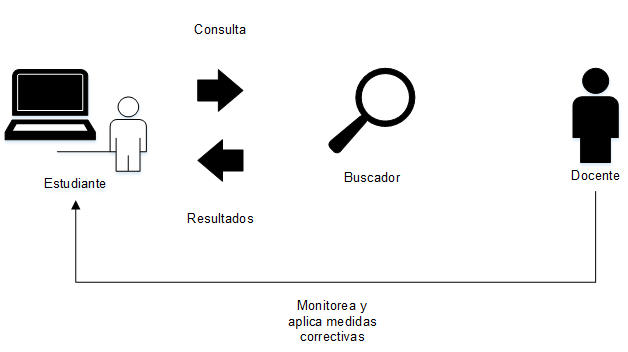
\includegraphics[width=0.7\textwidth]{03_GraphicFiles/p07.png}
	%\input{03_GraphicFiles/p07.pdf}
	\captionsource{Proceso de búsqueda de información de un estudiante.}{\fuentePropia}
	\label{fig:docente_estudiante}
\end{figure}

%Fuente: https://tex.stackexchange.com/questions/4338/correctly-scaling-a-tikzpicture
\begin{figure}[htb]
	\centering
	%FIX: dont compile
	%\scalebox{0.8}{%\centering\makebox[\textwidth]{
\begin{tikzpicture}[node distance=3cm, auto]

    % Place nodes
    \node[label={Estudiante},charlie,monitor,minimum size=1.3cm] (estudiante);
    \node[block, right of=estudiante] (data-ingestion) {Entrada de datos};
    \node[block, right of=data-ingestion] (data-clean) {Transformación de datos};
    \node[block, right of=data-clean] (model-training) {Entrenamiento del modelo};
    \node[block, right of=model-training] (model-testing) {Evaluación del modelo};
    \node[block, right of=model-testing] (prediction) {Predicción};

\draw[line] (estudiante) -- (data-ingestion)
            (data-ingestion) -- (data-clean)
            (data-clean) -- (model-training)
            (model-training) -- (model-testing)
            (model-testing) -- (prediction);

\path[line,dashed] 
   (model-testing.south) -- +(0,-.35) -| (model-training.south)
   (prediction.south) -- +(0,-.60) -| (data-ingestion.south);

\coordinate[below=11mm of data-ingestion] (bottom brace);

\draw [my brace]
      (data-ingestion.south|-bottom brace) -- (model-training.south west|-bottom brace) 
      node[bottom label] {
        %Obtención de datos de NEURONE
        \begin{itemize}
        \item Spark
        \end{itemize}
      };

\draw [my brace]
      (model-training.south|-bottom brace) -- (prediction.south west|-bottom brace) 
      node[bottom label] {
        %Environmental \& Human factors
        \begin{itemize}
        \item Spark ML
        \end{itemize}
      };


\end{tikzpicture}
%}
	%\resizebox{1.0\textwidth}{!}{%\centering\makebox[\textwidth]{
\begin{tikzpicture}[node distance=3cm, auto]

    % Place nodes
    \node[label={Estudiante},charlie,monitor,minimum size=1.3cm] (estudiante);
    \node[block, right of=estudiante] (data-ingestion) {Entrada de datos};
    \node[block, right of=data-ingestion] (data-clean) {Transformación de datos};
    \node[block, right of=data-clean] (model-training) {Entrenamiento del modelo};
    \node[block, right of=model-training] (model-testing) {Evaluación del modelo};
    \node[block, right of=model-testing] (prediction) {Predicción};

\draw[line] (estudiante) -- (data-ingestion)
            (data-ingestion) -- (data-clean)
            (data-clean) -- (model-training)
            (model-training) -- (model-testing)
            (model-testing) -- (prediction);

\path[line,dashed] 
   (model-testing.south) -- +(0,-.35) -| (model-training.south)
   (prediction.south) -- +(0,-.60) -| (data-ingestion.south);

\coordinate[below=11mm of data-ingestion] (bottom brace);

\draw [my brace]
      (data-ingestion.south|-bottom brace) -- (model-training.south west|-bottom brace) 
      node[bottom label] {
        %Obtención de datos de NEURONE
        \begin{itemize}
        \item Spark
        \end{itemize}
      };

\draw [my brace]
      (model-training.south|-bottom brace) -- (prediction.south west|-bottom brace) 
      node[bottom label] {
        %Environmental \& Human factors
        \begin{itemize}
        \item Spark ML
        \end{itemize}
      };


\end{tikzpicture}
%}}
	%Este funciona
	%%\centering\makebox[\textwidth]{
\begin{tikzpicture}[node distance=3cm, auto]

    % Place nodes
    \node[label={Estudiante},charlie,monitor,minimum size=1.3cm] (estudiante);
    \node[block, right of=estudiante] (data-ingestion) {Entrada de datos};
    \node[block, right of=data-ingestion] (data-clean) {Transformación de datos};
    \node[block, right of=data-clean] (model-training) {Entrenamiento del modelo};
    \node[block, right of=model-training] (model-testing) {Evaluación del modelo};
    \node[block, right of=model-testing] (prediction) {Predicción};

\draw[line] (estudiante) -- (data-ingestion)
            (data-ingestion) -- (data-clean)
            (data-clean) -- (model-training)
            (model-training) -- (model-testing)
            (model-testing) -- (prediction);

\path[line,dashed] 
   (model-testing.south) -- +(0,-.35) -| (model-training.south)
   (prediction.south) -- +(0,-.60) -| (data-ingestion.south);

\coordinate[below=11mm of data-ingestion] (bottom brace);

\draw [my brace]
      (data-ingestion.south|-bottom brace) -- (model-training.south west|-bottom brace) 
      node[bottom label] {
        %Obtención de datos de NEURONE
        \begin{itemize}
        \item Spark
        \end{itemize}
      };

\draw [my brace]
      (model-training.south|-bottom brace) -- (prediction.south west|-bottom brace) 
      node[bottom label] {
        %Environmental \& Human factors
        \begin{itemize}
        \item Spark ML
        \end{itemize}
      };


\end{tikzpicture}
%}
	%\input{03_GraphicFiles/p06.pdf}
	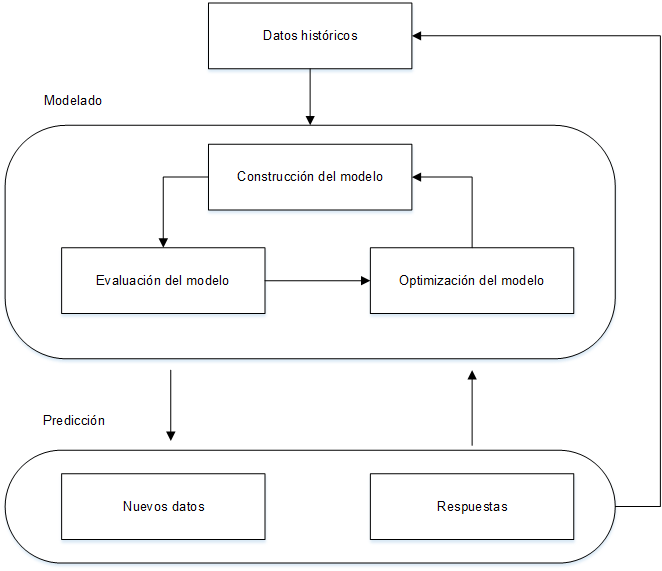
\includegraphics[width=0.7\textwidth]{03_GraphicFiles/p06.png}
	\captionsource{Ciclo de construcción y perfecionamiento del modelo.}{\fuentePropia}
	\label{fig:ml-pipeline}
\end{figure}


